
\newcommand{\gridthing}[3]{ 




\pgfmathtruncatemacro\fend{#1/2-1} 

\foreach \s in {0,...,\fend}{
    \pgfmathtruncatemacro\xpos{#2-#1/2+\s*2} 
    \filldraw[fill=white] (\xpos,#3-1) rectangle (\xpos+1,#3);
}

\foreach \s in {0,...,\fend}{
    \pgfmathtruncatemacro\xpos{#2-#1/2+\s*2} 
    \filldraw[fill=gray!10] (\xpos+1,#3-1) rectangle (\xpos+2,#3);
}

}

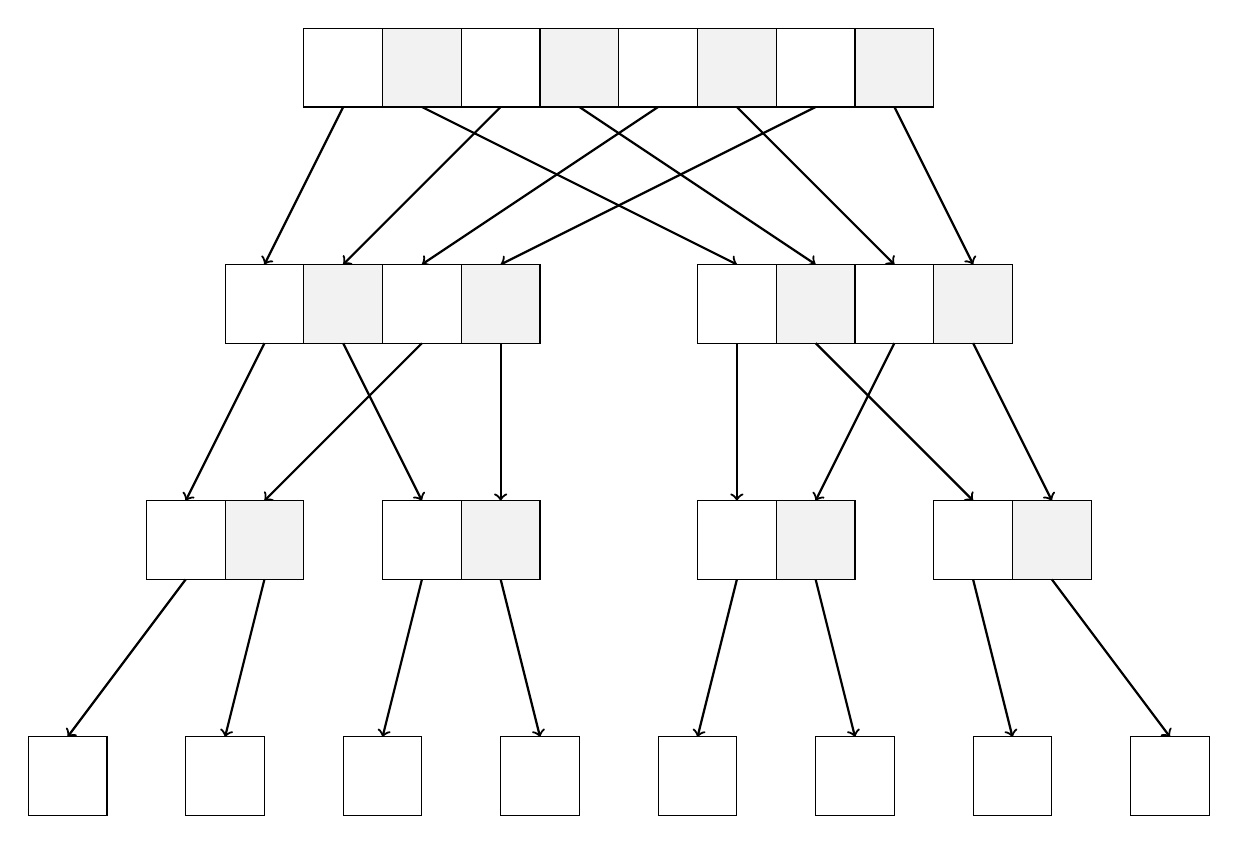
\begin{tikzpicture}[level/.style={sibling distance=60mm/#1}]

\gridthing{8}{0}{9}

\draw[thick,->] (-3.5,8) -- (-4.5,6);
\draw[thick,->] (-1.5,8) -- (-3.5,6);
\draw[thick,->] (0.5,8) -- (-2.5,6);
\draw[thick,->] (2.5,8) -- (-1.5,6);

\draw[thick,->] (3.5,8) -- (4.5,6);
\draw[thick,->] (1.5,8) -- (3.5,6);
\draw[thick,->] (-0.5,8) -- (2.5,6);
\draw[thick,->] (-2.5,8) -- (1.5,6);

\gridthing{4}{-3}{6}
\gridthing{4}{3}{6}

\draw[thick,->] (-4.5,5) -- (-5.5,3);
\draw[thick,->] (-3.5,5) -- (-2.5,3);
\draw[thick,->] (-2.5,5) -- (-4.5,3);
\draw[thick,->] (-1.5,5) -- (-1.5,3);

\draw[thick,->] (4.5,5) -- (5.5,3);
\draw[thick,->] (3.5,5) -- (2.5,3);
\draw[thick,->] (2.5,5) -- (4.5,3);
\draw[thick,->] (1.5,5) -- (1.5,3);

\gridthing{2}{-5}{3}
\gridthing{2}{-2}{3}
\gridthing{2}{2}{3}
\gridthing{2}{5}{3}

\draw[thick,->] (-5.5,2) -- (-7,0);
\draw[thick,->] (-4.5,2) -- (-5,0);
\draw[thick,->] (-2.5,2) -- (-3,0);
\draw[thick,->] (-1.5,2) -- (-1,0);

\draw[thick,->] (5.5,2) -- (7,0);
\draw[thick,->] (4.5,2) -- (5,0);
\draw[thick,->] (2.5,2) -- (3,0);
\draw[thick,->] (1.5,2) -- (1,0);

\foreach \l in {0,...,7}{
    \filldraw[fill=white] (\l*2-7.5,0) rectangle (\l*2-6.5,-1);
}

%\foreach \l in {8,4,2}{
%    \pgfmathtruncatemacro\basexpos{\l} 
%    \pgfmathtruncatemacro\ypos{ln(\l)/ln(2)} 
%
%    \pgfmathtruncatemacro\items{4-\ypos} 
%    \foreach \b in {1,...,\items}{
%        \pgfmathtruncatemacro\xposs{\basexpos*(\b-1)} 
%        \gridthing{\basexpos}{\xposs}{\ypos*3}
%     }
%}



%\gridthing{4}{1}{3}


\end{tikzpicture}
